\chapter{XIBO-Server}
\section{Beschreibung}
\begin{figure}[H]
\centering
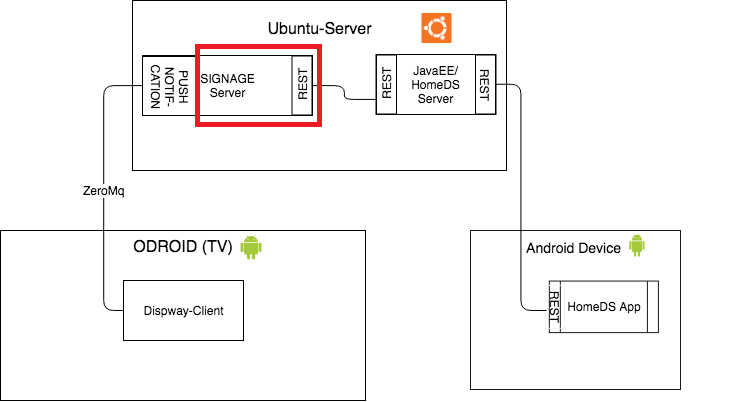
\includegraphics[width=1.0\textwidth]{images/03_XIBO-Server/03_SystemArch}
\caption{Systemkomponente XIBO-Server}
\label{fig:mediaNav}
\end{figure}

Als zentrale Steuereinheit wird ein XIBO-Server verwendet. Der XIBO-Server bietet die benötigten Funktionalitäten wie zum Beispiel:
\begin{itemize}
	\item {\em Medieninhalte abspielen} 
	\item {\em Zeitsteuerung der anzuzeigenden Informationen}  
	\item {\em Verteilung der Anzeigedaten an die verbundenen Clients} 
\end{itemize}
Es gibt zwei Möglichkeiten den Funktionsumfang des XIBO-Servers zu nutzen. Zum einen über das Server interne Web-Interface, zum anderen hat man die  Möglichkeit den Server über die eingebaute REST-Schnittstelle anzusprechen.(Siehe Abbildung \ref{fig:structXibo})
\cite{xibo-server}
\section{API}
\begin{figure}[H]
\centering
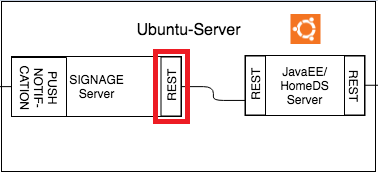
\includegraphics[width=1.0\textwidth]{images/03_XIBO-Server/03_XiboApi}
\caption{Gliederung Ubuntu-Server}
\label{fig:structXibo}
\end{figure}
Die API des XIBO-Servers ist mittels Swagger dokumentiert. Diese Dokumentation deckt die Grundfunktionalitäten und die Form der Anfragen ab. Die Schnittstelle des Servers dient als wesentliches Verbindungsstück zwischen der eigens entwickelten Steuerungssoftware und dem XIBO-Server. Wie der XIBO-Server die verschiedenen Anfragen verarbeitet und entgegen nimmt, wird, bevor die Implementierung des Java-EE-Servers beginnt, mittels Postman getestet. Diese Vorgehensweise ist Nötig um festzustellen, ob das XIBO-System über REST-API ausreichend konfigurierbar und im operativen Betrieb steuerbar ist. Die Anfragen an den Server werden im Java Code durch die ''libary'' OkHttp3 übernommen.\cite{swagger}\cite{postman}\cite{OkHttp3}

\section{Authentifizierung}
Die Authentifizierung einer Client-Applikation per REST-Anfrage am XIBO-Server erfolgt über OAuth2 , also mittels Access Token. \cite{oAuth2}

Zunächst ist am XIBO-Server ein ''Application''-Objekt im Webinterface zu erstellen. Beim Erstellen des ''Application''-Objekts können die Berechtigungen für den Client festgelegt werden. Nachdem das Objekt erstellt wird, stellt dieses ein ''Client Secret'' zur Verfügung. Dieses ist für jeden Client eindeutig.(Siehe Abbildung \ref{fig:base} und \ref{fig:permis} )
\begin{figure}[H]
\centering
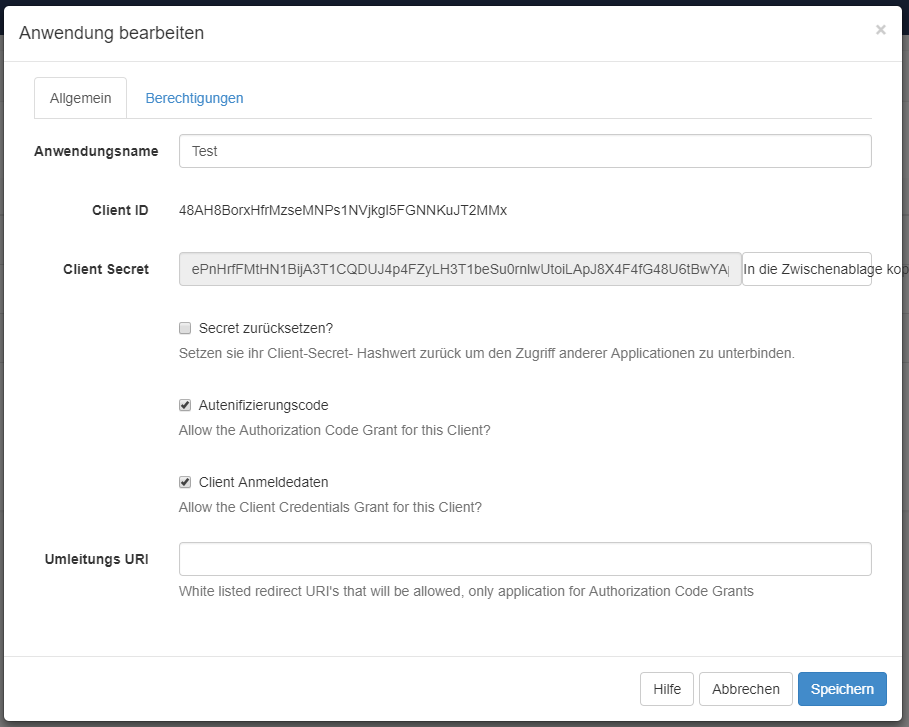
\includegraphics[width=1.0\textwidth]{images/03_XIBO-Server/03_EditApplikation}
\caption{Grundeinstellungen einer XIBO-Anwendung}
\label{fig:base}
\end{figure}
\begin{figure}[H]
\centering
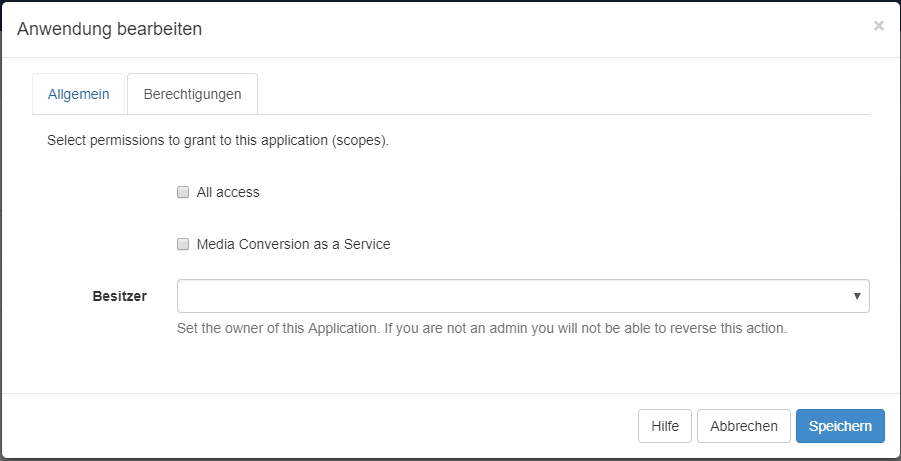
\includegraphics[width=1.0\textwidth]{images/03_XIBO-Server/03_ApplikationPermission}
\caption{Mögliche Berechtigungen für eine Xibo-Anwendung}
\label{fig:permis}
\end{figure}

Damit ein externer Client auf den XIBO-Server per REST-Request zugreifen beziehungsweise Anweisungen an diesen geben kann, wird ein POST-Request mit folgenden Parametern abgesetzt.

Die Parameter: 
\begin{itemize}
	\item {\em Client\_ID:} Wird vom XIBO-Server bereitgestellt
	\item {\em Client\_Secret:} Wird vom XIBO-Server bereitgestellt
	\item{\em grant\_type:} Muss in der Form ''&grant\_type=client\_credentials''
\end{itemize}

Die über den POST-Request erhaltene Antwort, liefert einen Access Token, welcher 60 Minuten gültig ist und nach Ablauf erneuert werden muss, um weiter über die API zu kommunizieren.
Dieser Token muss bei jedem Request an den XIBO-Server im Header des Requests übergeben werden, damit der XIBO-Server feststellen kann, ob es sich um einen registrierten Client handelt.


Um die Authentifizierung zu automatisieren, wurde eine Java Klasse entwickelt, diese ist zu finden im HomeDsBackend (HomeDS/HomeDsBackend/src/main/java/at/htl/utils/AuthentificationHandler.java). Funktionsweise dieser wird nachfolgend geschildert: 

Um eine Verbindung zum XIBO-Server herstellen zu können wird eine URL und eine HttpURLConnection deklariert. Im Anschluss wird die URL mit der richtigen Adresse belegt. Die httpURLConnection wird über den Befehl ''httpURLConnection.openConnection()'' dazu angewiesen, eine Verbindung aufzubauen. Durch die Anweisung ''httpURLConnection.setDoOutput(true)'' wird der Connection mitgeteilt, dass als Antwort Daten erhalten werden. Die Art der Anfrage wird als POST-Request festgelegt.  \citep{httpurlconnection}

\begin{lstlisting}[language=Java,caption={Erstellen der Verbindung zum Server}]
URL obj;
HttpURLConnection con = null;
	try {
    	// Building Connection
        obj = new URL(new RequestHelper()
        	.BASE_URL + AUTHORIZE_URL);
       	con = (HttpURLConnection) obj.openConnection();
        con.setRequestProperty("Content-Type",
             "application/x-www-form-urlencoded");    
        con.setDoOutput(true);
        con.setRequestMethod("POST");
\end{lstlisting}

Um die für die Authentifizierung am XIBO-Server geforderten Parameter ''client\_id'', ''client\_secret'' und ''grant\_type'' übergeben zu können wird ein ''DataOutputStream'' deklariert und mit den benötigten Werten versehen. Anschließend wird über den Befehl  ''DataoutputStrem.flush'' dem ''DataOutputStream'' mitgeteilt, dass er die Daten über die Verbindung senden soll.
\begin{lstlisting}[language=Java,caption={Erstellen und senden des JSON-Body}]
DataOutputStream write 
	= new DataOutputStream(con.getOutputStream());
	 
String body = "client_id=" + CLIENT_ID
              + "&client_secret=" + CLIENT_SECRET
              + "&grant_type=client_credentials";

write.writeBytes(body);
write.flush();
\end{lstlisting}

Um auftretende Fehler besser finden zu können, werden der übergebene Request-Body, die URL über die der Request durchgeführt wurde und der erhaltene Response-Code im Log-Fenster ausgegeben. Die Daten, die anschließend vom XIBO-Server als Antwort erhalten werden, werden durch einen ''BufferedReader'', dieser bekommt bei der Instanziierung den ''InputStream'' der ''httpURLConnection'' übergeben, entgegengenommen. Solange vom Server Daten erhalten werden, wird über einen ''StringBuilder'' ein String um jene erhaltenen Daten erweitert. Im Anschluss wird die ''BufferedReader'' Verbindung geschlossen und der erhaltene ''Access\_Token'' wird im Log-Fenster angezeigt.

\begin{lstlisting}[language=Java,caption={Erhalt der Daten vom Server}]
System.out.println("nPost-Body: " + body);
System.out.println("nSending 'AUTHORIZATION'
    request to URL : " + AUTHORIZE_URL);
             
System.out.println("Response Code :
				" + con.getResponseCode());

BufferedReader in = new BufferedReader(
    new InputStreamReader(con.getInputStream()));
    
String output;
StringBuilder response = new StringBuilder();
while ((output = in.readLine()) != null) {
        response.append(output);
}
\end{lstlisting}

Als nächstes wird der erhaltene Token per ''return'' Statement als Ergebnis der Methode übergeben. Abschließend wird im ''finally'' Block überprüft, ob die ''HttpURLConnection'' noch geöffnet beziehungsweise vorhanden ist. Sollte dies der Fall sein so wird die Verbindung geschlossen.
\begin{lstlisting}[language=Java,caption={Rückgabe des Token und schließen der Verbindung}]
	in.close();
	System.out.println(response.toString());

	return new JSONObject(
     	response.toString()).getString("access_token");
     	
} catch (MalformedURLException e) {
	e.printStackTrace();
} catch (IOException e) {
    e.printStackTrace();
}
finally {
	if (con != null)
    	con.disconnect();
}
\end{lstlisting}




